\documentclass[pdflatex]{article}
%These tell TeX which packages to use.

\usepackage{array,epsfig}
\usepackage{amsmath}
\usepackage{amsfonts}
\usepackage{amssymb}
\usepackage{amsxtra}
\usepackage{amsthm}
\usepackage{mathrsfs}
\usepackage{color}
\usepackage[margin=2cm,top=2.5cm,headheight=16pt,headsep=0.1in,heightrounded]{geometry}
\usepackage{fancyhdr}
\pagestyle{fancy}
\usepackage{tikz}
\usepackage{graphics}
\usepackage{float}
\usepackage{sistyle}
\usepackage[utf8]{inputenc}      % accents dans le source
\usepackage[T1]{fontenc}
\usepackage[francais]{babel}
\usepackage{verbatim}

\setlength{\textheight}{24cm} % Hauteur de la zone de texte
\setlength{\textwidth}{17cm} % Largeur de la zone de texte
\setlength{\topmargin}{-0.8cm}  % marge en haut
\setlength{\oddsidemargin}{-0.5cm} % Marge gauche sur pages impaires (book) quelconques (article)
\setlength{\headheight}{1cm} % Haut de page
\setlength{\headsep}{3mm} % Entre le haut de page et le texte
\setlength{\footskip}{1cm} % Bas de page + séparation

%Here I define some theorem styles and shortcut commands for symbols I use often
\theoremstyle{definition}
\newtheorem{defn}{Definition}
\newtheorem{thm}{Theorem}
\newtheorem{cor}{Corollary}
\newtheorem*{rmk}{Remark}
\newtheorem{lem}{Lemma}
\newtheorem*{joke}{Joke}
\newtheorem{ex}{Example}
\newtheorem*{soln}{Solution}
\newtheorem{prop}{Proposition}

\newcommand{\lra}{\longrightarrow}
\newcommand{\ra}{\rightarrow}
\newcommand{\surj}{\twoheadrightarrow}
\newcommand{\graph}{\mathrm{graph}}
\newcommand{\bb}[1]{\mathbb{#1}}
\newcommand{\Z}{\bb{Z}}
\newcommand{\Q}{\bb{Q}}
\newcommand{\R}{\bb{R}}
\newcommand{\E}{\bb{E}}
\newcommand{\C}{\bb{C}}
\newcommand{\N}{\bb{N}}
\newcommand{\Pe}{\bb{P}}
\newcommand{\M}{\mathbf{M}}
\newcommand{\m}{\mathbf{m}}
\newcommand{\MM}{\mathscr{M}}
\newcommand{\HH}{\mathscr{H}}
\newcommand{\Om}{\Omega}
\newcommand{\Ho}{\in\HH(\Om)}
\newcommand{\bd}{\partial}
\newcommand{\del}{\partial}
\newcommand{\bardel}{\overline\partial}
\newcommand{\textdf}[1]{\textbf{\textsf{#1}}\index{#1}}
\newcommand{\img}{\mathrm{img}}
\newcommand{\ip}[2]{\left\langle{#1},{#2}\right\rangle}
\newcommand{\inter}[1]{\mathrm{int}{#1}}
\newcommand{\exter}[1]{\mathrm{ext}{#1}}
\newcommand{\cl}[1]{\mathrm{cl}{#1}}
\newcommand{\ds}{\displaystyle}
\newcommand{\vol}{\mathrm{vol}}
\newcommand{\cnt}{\mathrm{ct}}
\newcommand{\osc}{\mathrm{osc}}
\newcommand{\LL}{\mathbf{L}}
\newcommand{\UU}{\mathbf{U}}
\newcommand{\support}{\mathrm{support}}
\newcommand{\AND}{\;\wedge\;}
\newcommand{\OR}{\;\vee\;} 
\newcommand{\Oset}{\varnothing}
\newcommand{\st}{\ni}
\newcommand{\wh}{\widehat}
\newcommand{\vect}[1]{\overrightarrow{#1}}
\newcommand{\quest}[1]{\textbf{\textit{#1}} \vspace{3mm}}

%Pagination stuff.
%\setlength{\oddsidemargin}{0in}
%\setlength{\evensidemargin}{0in}
%\setlength{\textheight}{9.in}
%\setlength{\textwidth}{6.5in}
%\cfoot{page \thepage}
\lhead{MEU359 - Proba-Stat}
\rhead{TP}
\pagestyle{fancy}


\begin{document}
\title{R\'egression linr\'eaire pour mesurer la hauteur des eucalyptus}

\author{Charlote Ayrault - The ghost}
\date{\today}


\maketitle

\section*{R\'egression lin\'eaire simple}
\subsection*{Question 1}
\quest{Pourquoi proposer un estimateur lin\'eaire simple?}

On voit clairement sur le nuage de points (circonference/hauteur) que cela suit une droite. On essaye de trouver les valeurs de la droites qui minimisent le risque quadratique.

\subsection*{Question 2}
\quest{Comment minimise-t-on une fonction de deux variables? Trouver $\hat{\beta_1}$ et $\hat{\beta_2}$?}

Pour minimiser la fonction $\varphi(\beta_1, \beta_2)$ il faut trouver d\'eriver la fonction par rapport \`a $\beta_1$ et $\beta_2$ et trouver les valeurs qui annulent les 2 d\'eriv\'ees.
$$
\frac{\partial \varphi(\beta_1, \beta_2)}{\beta_1} = \frac{\sum_{i=1}^{n}{(Y_i - \beta_1 - \beta_2x_i)^2}}{\beta_1} = \frac{\sum_{i=1}^{n}{Y_i^2 - \beta_1Y_i - \beta_2x_iY_i -\beta_1Y_i + \beta_1^2 + \beta_1\beta_2x_i - \beta_2x_iY_i + \beta_2x_i\beta_1 +\beta_2^2x_i^2}}{\beta_1}
$$
$$
= \sum_{i=1}^{n}{-Y_i -Y_i +2\beta_1 +\beta_2x_i+\beta_2x_i} = 2 \sum_{i=1}^{n}{-Y_i+\beta_2x_i+\beta_1}
$$
$$
\frac{\partial \varphi(\beta_1, \beta_2)}{\beta_2} = \frac{\sum_{i=1}^{n}{(Y_i - \beta_1 - \beta_2x_i)^2}}{\beta_2} = \frac{\sum_{i=1}^{n}{Y_i^2 - \beta_1Y_i - \beta_2x_iY_i -\beta_1Y_i + \beta_1^2 + \beta_1\beta_2x_i - \beta_2x_iY_i + \beta_2x_i\beta_1 +\beta_2^2x_i^2}}{\beta_2}
$$
$$
= \sum_{i=1}^{n}{-x_iY_i+\beta_1x_i-x_iY_i + \beta_1x_i+2\beta_2x_i^2} = 2 \sum_{i=1}^{n}{x_i(-Y_i+\beta_2x_i+\beta_1)}
$$

On cherche $\hat{\beta_1}$ et $\hat{\beta_2}$ les valeurs qui annulent le syst\`eme
$$
\left\{
\begin{array}{l}
\sum_{i=1}^{n}{x_i(-Y_i+\beta_2x_i+\beta_1)} = 0 \\
\sum_{i=1}^{n}{-Y_i+\beta_2x_i+\beta_1} = 0
\end{array}
\right.
$$
$$
\left\{
\begin{array}{l l}
\sum_{i=1}^{n}{-Y_ix_i}+\sum_{i=1}^{n}{\beta_2x_i^2}+\sum_{i=1}^{n}{\beta_1x_i} = 0 & (1)\\
\sum_{i=1}^{n}{-Y_i} +\sum_{i=1}^{n}{\beta_2x_i}+\sum_{i=1}^{n}{\beta_1} = 0 & (2)
\end{array}
\right.
$$
$$
\left\{
\begin{array}{l l}
\sum_{i=1}^{n}{-Y_ix_i}+\beta_2\sum_{i=1}^{n}{x_i^2}+\beta_1\sum_{i=1}^{n}{x_i} = 0 & (1)\\
\sum_{i=1}^{n}{-Y_i} +\beta_2\sum_{i=1}^{n}{x_i}+n\beta_1 = 0 & (2)
\end{array}
\right.
$$


On fait $(3) = n(1)-(2)\sum_{i=1}^{n}{x_i}$
$$
\left\{
\begin{array}{l l}
n\sum_{i=1}^{n}{-Y_ix_i}+n\beta_2\sum_{i=1}^{n}{x_i^2}+\sum_{i=1}^{n}{Y_i}\sum_{i=1}^{n}{x_i} -\beta_2\left(\sum_{i=1}^{n}{x_i}\right)^2 = 0 & (3)\\
\sum_{i=1}^{n}{-Y_i} +n\beta_2\sum_{i=1}^{n}{x_i}+n\beta_1 = 0 & (2)
\end{array}
\right.
$$
$$
\left\{
\begin{array}{l l}
-n\sum_{i=1}^{n}{Y_ix_i} + \sum_{i=1}^{n}{Y_i}\sum_{i=1}^{n}{x_i} = \beta_2\left(\sum_{i=1}^{n}{x_i}\right)^2 -n\beta_2\sum_{i=1}^{n}{x_i^2}  & (3)\\
\sum_{i=1}^{n}{-Y_i} +n\beta_2\sum_{i=1}^{n}{x_i}+n\beta_1 = 0 & (2)
\end{array}
\right.
$$
$$
\left\{
\begin{array}{l l}
\beta_2 = \frac{\sum_{i=1}^{n}{Y_i}\sum_{i=1}^{n}{x_i}-n\sum_{i=1}^{n}{Y_ix_i}}{\left(\sum_{i=1}^{n}{x_i}\right)^2 -n\sum_{i=1}^{n}{x_i^2}}  & (3)\\
\beta_1 = \frac{1}{n}(\sum_{i=1}^{n}{Y_i} - n\beta_2\sum_{i=1}^{n}{x_i}) & (2)
\end{array}
\right.
$$
$$
\left\{
\begin{array}{l l}
\beta_2 = \frac{\sum_{i=1}^{n}{Y_i}\sum_{i=1}^{n}{x_i}-n\sum_{i=1}^{n}{Y_ix_i}}{\left(\sum_{i=1}^{n}{x_i}\right)^2 -n\sum_{i=1}^{n}{x_i^2}}  & (3)\\
\beta_1 = \frac{\sum_{i=1}^{n}{x_i}\sum_{i=1}^{n}{x_iY_i}-\sum_{i=1}^{n}{x_i^2}\sum_{i=1}^{n}{Y_i}}{\left(\sum_{i=1}^{n}{x_i}\right)^2 -n\sum_{i=1}^{n}{x_i^2}} & (2)
\end{array}
\right.
$$

\subsection*{Question 3}
\quest{Programmer et tracer la droite de r\'egression $y = \hat{\beta_1} + \hat{\beta_2}x$?}

Voir la figure ~\ref{fig:regression simple}.
\begin{figure}
	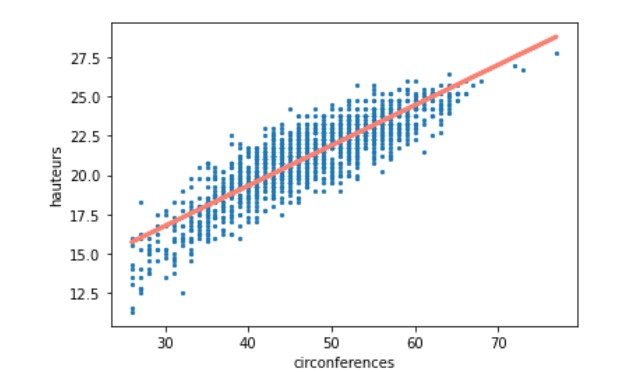
\includegraphics[scale=1]{regression_simple.jpg}
    \caption{R\'egression simple}
    \label{fig:regression simple}
\end{figure}

On a obtenu $\hat{\beta_1} =  9.037475668452768$  et $\hat{\beta_2} = 0.257137855007109$.

\begin{itemize}
    \item Moyenne de espilon: -3.603610217941441e-11
    \item risque quadratique: 19.492804231375466
\end{itemize}
    
\subsection*{Question 4}
\quest{Que pensez-vous de ces hypoth\`eses ? Comment peut-on estimer ce param\`etre de variance $\sigma^2$ ?}

Comme le montre les figures \ref{fig:Circonference} et \ref{fig:Hauteur}, il semble raisonnable de dire que la circonf\'erence (resp. la hauteur) d'un eucalyptus suit une loi normale. Maintenant on n'a qu'un seul \'echantillon, donc cela pourrait \^etre une pure coincidence!

\begin{figure}
    \centering
    \begin{minipage}{0.45\textwidth}
        \centering
            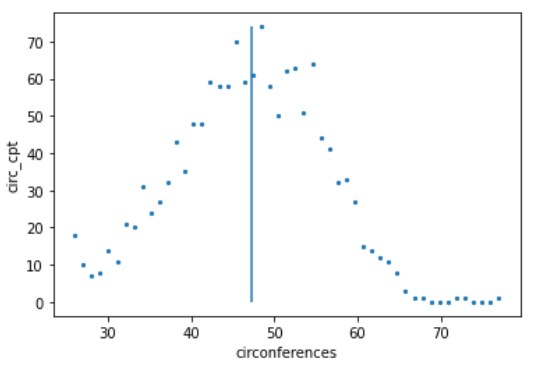
\includegraphics[scale=0.5]{circ_normale.jpg}
            \caption{Circonference}
            \label{fig:Circonference}
    \end{minipage}\hfill
    \begin{minipage}{0.45\textwidth}
        \centering
        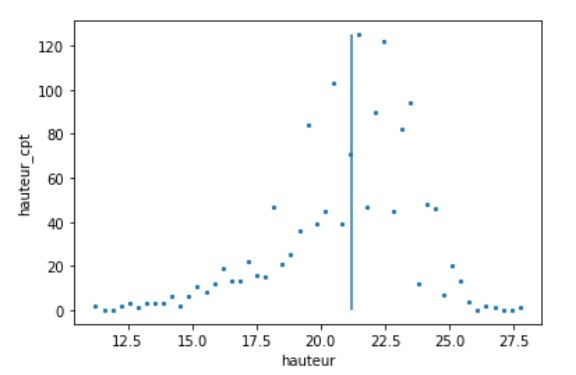
\includegraphics[scale=0.5]{hauteur_normale.jpg}
        \caption{Hauteur}
        \label{fig:Hauteur}
    \end{minipage}
\end{figure}


Comme les 2 variables al\'eatoires suivent une loi normale, elle sont ind\'ependentes et identiquement distribu\'es.

Si X suit une loi normale $\mathscr{N}(m, \sigma^2)$ et $Y = AX + b$ alors, $Y$ suit une loi normale $\mathscr{N}(am + b, a^2\sigma^2)$  

Si $X$ (resp. $Y$) suit une loi normale $\mathscr{N}(m_x, \sigma_x^2)$ (resp. $\mathscr{N}(m_y, \sigma_y^2)$) alors $X+Y$ suit une loi normale $\mathscr{N}(m_x + m_y, \sigma_x^2+\sigma_y^2)$.

Dans notre cas on a $e_i = Y_i - \hat{\beta_1} + \hat{\beta_2}x_i$. Donc $e_i$ suit une loi normale  
$\mathscr{N}(- \hat{\beta_1} - \hat{\beta_2}m_x + m_Y, \hat{\beta_2}^2\sigma_x^2+\sigma_y^2)$. On a par d\'efinition $m_y = \hat{\beta_1} + \hat{\beta_2}m_x$. Donc $E(e_i) = 0$ et $\sigma_{e_i} = \hat{\beta_2}^2\sigma_x^2+\sigma_y^2$.

\section*{R\'egression lin\'eaire multiple}
\subsection*{Question 5}
\quest{Montrer que $X\hat{\beta} = P_F(Y)$, o\`u $P_F(Y)$ est la projection orthonogale de $Y$ sur $F$. En d\'eduire : $\forall \theta \in \R^3, \langle Y - X\hat{\beta}, X\theta \rangle = 0$.}

En cherchant \`a minimiser $\lVert Y - X\beta \rVert^2$, on cherche \`a trouver l'\'el\'ement de $F$ le plus proche de $Y$ au sens de la distance euclidienne. Il s'agit de la projection orthogonale de $Y$ sur $F$. Comme $z \in F$, si et seulement si $z = X\beta$, on cherche $\hat{\beta}$ tel que $X\hat{\beta} = P_F(Y)$. 

Comme $X\hat{\beta} = P_F(Y)$, on a $Y - X\hat{\beta} = Y - P_F(Y)$ qui est un vecteur orthogonal \`a $X$ et par cons\'equent aussi a $X\theta$. Le produit scalaire de 2 vecteurs orthogonaux est nul, donc $\forall \theta \in \R^{3}, \langle Y - X\hat{\beta}, X\theta \rangle = 0$.

\subsection*{Question 6}
\quest{Montrer que $\hat{\beta} = (X^TX)^{-1}X^TY$.}

Pour trouver le minimum par rapport a $\beta$, il suffit de d\'eriver l'expression par rapport \`a $\beta$ et annuler l'expression. On remarque que $\sum_{i=1}^{n}{(Y-X\beta)^2} = (Y-X\beta)^t(Y-X\beta)$

$$
(Y-X\beta)^t(Y-X\beta) = (Y^t-\beta^tX^t)(Y-X\beta) = Y^tY-Y^tX\beta - \beta^tX^tY + \beta^tX^tX\beta
$$
et
$$
\frac{\partial (Y-X\beta)^t(Y-X\beta) }{\partial \beta} = -Y^tX + \beta^tX^tX
$$
On cherche $\hat{\beta}$ tel que
$$
-Y^tX + \hat{\beta}^tX^tX = 0
$$
$$
(\hat{\beta}^tX^tX)^t = (-Y^tX)^t
$$
Donc
$$
\hat{\beta} = (X^tX)^{-1}X^tY
$$

\subsection*{Question 7}
\quest{Programmer et tracer la courbe de r\'egression $\hat{\beta_1} + \hat{\beta_2}x + \hat{\beta_3}\sqrt{x}$.}

Voir figure \ref{fig:Regression multiple}.

\begin{figure}
	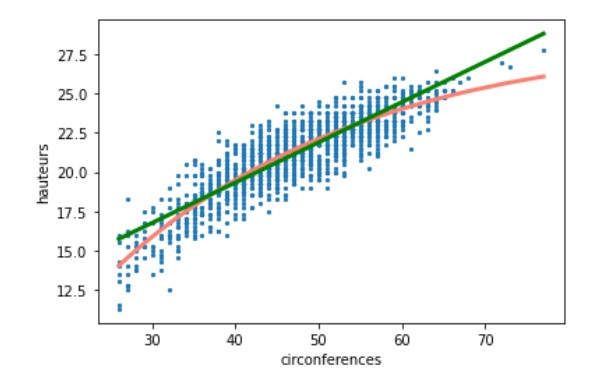
\includegraphics[scale=1]{regression_multiple.jpg}
    \caption{Regression multiple}
    \label{fig:Regression multiple}
\end{figure}

\vspace{5mm}
On a obtenu les valeurs suivantes:
\begin{itemize}
    \item $\hat{\beta_1} = -24.35200327$
    \item $\hat{\beta_2} = -0.48294547$
    \item $\hat{\beta_3} = 9.98688814$
\end{itemize}

\vspace{5mm}
On a \'egalement calcul\'e:
\begin{itemize}
    \item Moyenne de espilon: 1.0692449957862278e-13
    \item risque quadratique: 19.32298986873724
\end{itemize}

\vspace{5mm}
Les valeurs proches mais meilleures que celles de la r\'egression simple \`a la question 3.


\subsection*{Question 8}
\quest{Quel est alors la loi des $Y_i$ ? Montrer que $\hat{\beta}$ est l'estimateur du maximum de vraisemblance. Calculer la loi des $\hat{\beta_j}$.}

On suppose que $\epsilon_i \sim \mathscr{N}(0,\sigma^2)$ et on a $Y_i = X_i\beta + \epsilon_i$. La loi suivit par $Y_i$ d\'epend de la loi suivit par $X_i$ et $\beta$. Donc si on suppose que $X_i$ suit une loi exponentielle, il y a de grande chance que $Y_i$ suive aussi une loi exponentielle.

Maintenant, sur le seul \'echantillon fourni, on a montr\'e \`a la question 4 que $X_i$ suit certainement une loi normale (mais avec un seul \'echantillon on ne peut pas \^etre sur).


\section*{Test de Student}
Pourquoi on cherche \`a se demander si $\beta_3 = 0$. On fait la supposition ici que les $\beta_1$ et $\beta_2$ sont identiques pour les 2 types de r\'egression pour l'\'echantillon donn\'e. Ce qui n'est pas le cas.

Sur l'\'echantillon donn\'e la r\'egression multiple est meilleure. 

\subsection*{Question 9}
\quest{Montrer qur $T$ suit une loi de Student \`a $(n - 3)$ degr\'es de libert\'e $\tau (n - 3)$}

Soient Z une variable al\'eatoire de loi normale centr\'ee et r\'eduite et U une variable ind\'ependante de Z et distribu\'ee suivant la loi la loi du chi-deux \`a k degr\'es de libert\'e. Par d\'efinition la variable $T=\frac {Z}{\sqrt {U/k}}$ suit une loi de Student \`a k degr\'es de libert\'e.

Prenons $U = (n-3)\hat{\sigma}^2/\sigma^2$. On sait que $U$ suit une loi de chi-deux \`a $(n-3)$ degr\'es de libert\'e (voir question pr\'ec\'edente) et $Z = \frac{\hat{\beta_3}}{\sigma m_3}$ suit une loi normale centr\'ee et r\'eduite et $k = n-3$.

$$
\frac{Z}{\sqrt{\frac{U}{n-3}}} = \frac{\frac{\hat{\beta_3}}{\sigma m_3}}{\sqrt{\frac{(n-3)\hat{\sigma}^2/\sigma^2}{n-3}}}
= \frac{\hat{\beta_3}}{\sigma m_3 \frac{\hat{\sigma}}{\sigma}} 
= \frac{\hat{\beta_3}}{m_3 \hat{\sigma}} = T
$$


\subsection*{Question 10}
\quest{En d\'eduire une roc\'edure de test. L'impl\'ementer sur les donn\'es. Quelle conclusion pouvez-vous en tirer? Pourrait-on se passer de a composante lin\'eaire en $x$ de la r\'egression ?}

L'erreur de deviation standard de $Se(\hat{\beta_3}) = \sqrt{[(X^tX)^{-1}]_{3x3}\hat{\sigma}^2}$. la t-value pour le test est $\frac{\hat{\beta_3} - 0}{Se(\hat{\beta_3})}$ avec $\hat{\beta_3} = 9.98688814$, $[(X^tX)^{-1}]_{3x3} = $, $\hat{\sigma}^2 = $ et $Se(\hat{\beta_3}) = $.

Les coefficients $\hat{\beta_1}$ $\hat{\beta_2}$ de la r\'egression lin\'eaire simple et multiple sont diff\'erents donc on ne peut pas se passer de la composante $\sqrt{x}$ dans la r\'egression multiple car dans ce cas la regression simple associ\'ee ne donne pas le plus petit risque quadratique.  

\subsection*{Question 11}
\quest{Dans le cas de la r\'egression lin\'eaire simple, donner les intervalles de confiance a 95\% et 99\% pour $\beta_1$ et $\beta_2$. Les tracer en fonction de $n$ pour les donn\'ees fournies}

Les intervalles de confiance sont 
$$
\hat{\beta_0} \pm t_{\alpha/2;n-2}\sqrt{\hat{\sigma}^2\left(\frac{1}{n}+\frac{\bar{X}^2}{\sum_{i=1}^{n}{(X_i-\bar{X})^2}}\right)}
$$
$$
\hat{\beta_1} \pm t_{\alpha/2;n-2}\sqrt{\frac{\hat{\sigma}^2}{\sum_{i=1}^{n}{(X_i-\bar{X})^2}}}
$$

Voir programme python.

Intervalle de confiance \`a 95\% de $\hat{\beta_0} = -0.14857451813593908$, celui de $\hat{\beta_1} = -0.007332356088614205$.  Donc, $ \hat{\beta_0} \in [8.888901150316945, 9.186050186588824]$ et $\hat{\beta_1} \in [0.24980549891849463, 0.26447021109572305]$.

Intervalle de confiance \`a 99\% de $\hat{\beta_0} = -0.19535568338512507$, celui de $\hat{\beta_1} = -0.009641070706375857$. Donc, $ \hat{\beta_0} \in [8.84211998506776, 9.23283135183801]$ et $\hat{\beta_1} \in [0.247496784300733, 0.2667789257134847]$.

\vspace{5mm}
On n'a pas pu les tracer en fonction de $n$ car cela d\'epend des $n$ donn\'ees que l'on prend pour faire le calcul. 

\section*{Estimateur de la variance}
\subsection*{Question 12}
\quest{Montrer que $AU + b \thicksim \mathcal{N}(Am + b, A\Sigma A^T)$.}

Par lin\'earit\'e de l'esp\'erance on a $E[AX+b] = AE[X] + b$]. Pour la variance on a 
$$
VAR(AX+b) = VAR(AX) = E[(AX)(AX)^t] = E[AXX^tA^t] = AE[XX^t]A^t = AVAR(X)A^t
$$

\subsection*{Question 13}
\quest{Montrer que $Y - X\hat{\beta}$ peut s'\'ecrire $P\epsilon$ o\`u $P$ est la matrice d'une projection orthogonale \`a pr\'eciser.}

On a $\hat{\beta} = (X^tX)^{-1}X^tY$ et $Y = X\beta + \epsilon$ donc

$$Y - X\hat{\beta} = Y - X(X^tX)^{-1}X^tY = (I_n - X(X^tX)^{-1}X^t)Y = (I_n - X(X^tX)^{-1}X^t)(X\beta +\epsilon) 
$$
$$
= X\beta - X(X^tX)^{-1}X^tX\beta + (I_n-X(X^tX)^{-1}X^t)\epsilon = X\beta - X\beta = (I_n - X(X^tX)^{-1}X^t)\epsilon
$$

Notons $H = X(X^tX)^{-1}X^t$, on a donc $P = (I_n - H)$.

\subsection*{Question 14}
\quest{D\'eterminer l'esp\'erance et la matrice de variance de $Y - X\hat{\beta}$.}

On a $E(Y-X\hat{\beta}) = E(P\epsilon) = PE(\epsilon) = P.0 = 0$.


\subsection*{Question 15}
\quest{En d\'eduire que $\hat{\sigma}^2$ est un estimateur sans biais de $\sigma^2$.}

Il faut montrer que $E(\hat{\sigma}^2)=\sigma^2$.


\subsection*{Question 16}
\quest{Montrer que $(n-3)\hat{\sigma}^2/\sigma^2 \thicksim \chi (n-3)$ et $\hat{\sigma}^2$ ind\'ependant de $\hat{\beta}$}

$$
(n-3)\frac{\hat{\sigma}^2}{\sigma^2} = \frac{\Vert Y - X\hat{\beta}\Vert^2}{\sigma^2} = \frac{\sum_{i=1}^{n}e_i}{\sigma^2} = \frac{e^te}{\sigma^2}
$$
Calculons $e^te$
$$
e^te = (P\epsilon)^t(p\epsilon) = \epsilon^t(I_n-H)^t(I_n - H)\epsilon = \epsilon^t(I_n - H)\epsilon
$$
Donc on a 
$$
(n-3)\frac{\hat{\sigma}^2}{\sigma^2} = \frac{\epsilon^t(I_n - H)\epsilon}{\sigma^2} = \frac{\epsilon^t}{\sigma}(I_n - H)\frac{\epsilon}{\sigma}
$$

En utilisant le th\'eor\`eme de Fisher Cochran, la formule ci-dessus a une distribution $\chi^2$ avec un degr\'es de libert\'e $rang(I_n-H)$.
$$
rang(I_n - H) = tr(I_n -H) = n - tr(H) = tr(X(X^tX)^{-1}X^t) = tr(I_3) = 3
$$
Donc 
$(n-3)\frac{\hat{\sigma}^2}{\sigma^2}$ a une distribution $\chi^2(n-3)$.


\section*{Best Linear Unbiased Estimator (BLUE)}

\subsection*{Question 17}
\quest{Interpr\'eter la propri\'et\'e $MSE_{\lambda}(\bar{\beta}) \leq MSE_{\lambda}(\tilde{\beta})$}

\subsection*{Question 18}
\quest{Montrer que, si $\tilde{\beta}$ est sans biais, alors $MSE_\lambda(\tilde{\beta}) = VAR[\lambda^T\tilde{\beta}]$. En d\'eduire que $\bar{\beta}$ est le BLUE si et seulement si, pout tout estimateur lin\'eaire sans biais $\tilde{\beta}$, $Var(\tilde{\beta}) - Var(\bar{\beta})$ est une matrice positive.}

\subsection*{Question 19}
\quest{En \'ecrivant $\tilde{\beta} = \hat{\beta} + DY = ((X^TX)^{-1}X^T+D)Y$, montrer $DX = 0$, puis $Var(\tilde{beta}) - Var(\hat{\beta})$ est positive. Conclure.}

\end{document}

